\begin{frame}[fragile]{\normalfont\jlv{PlutoPapers.jl}} \pause

\centering
\textit{What if we could interact directly with the code in research papers?}

\end{frame}


\begin{frame}[fragile]{\normalfont\jlv{PlutoPapers.jl}}

\begin{columns}
  \hfill
  \begin{column}{0.35\textwidth}
    \centering
    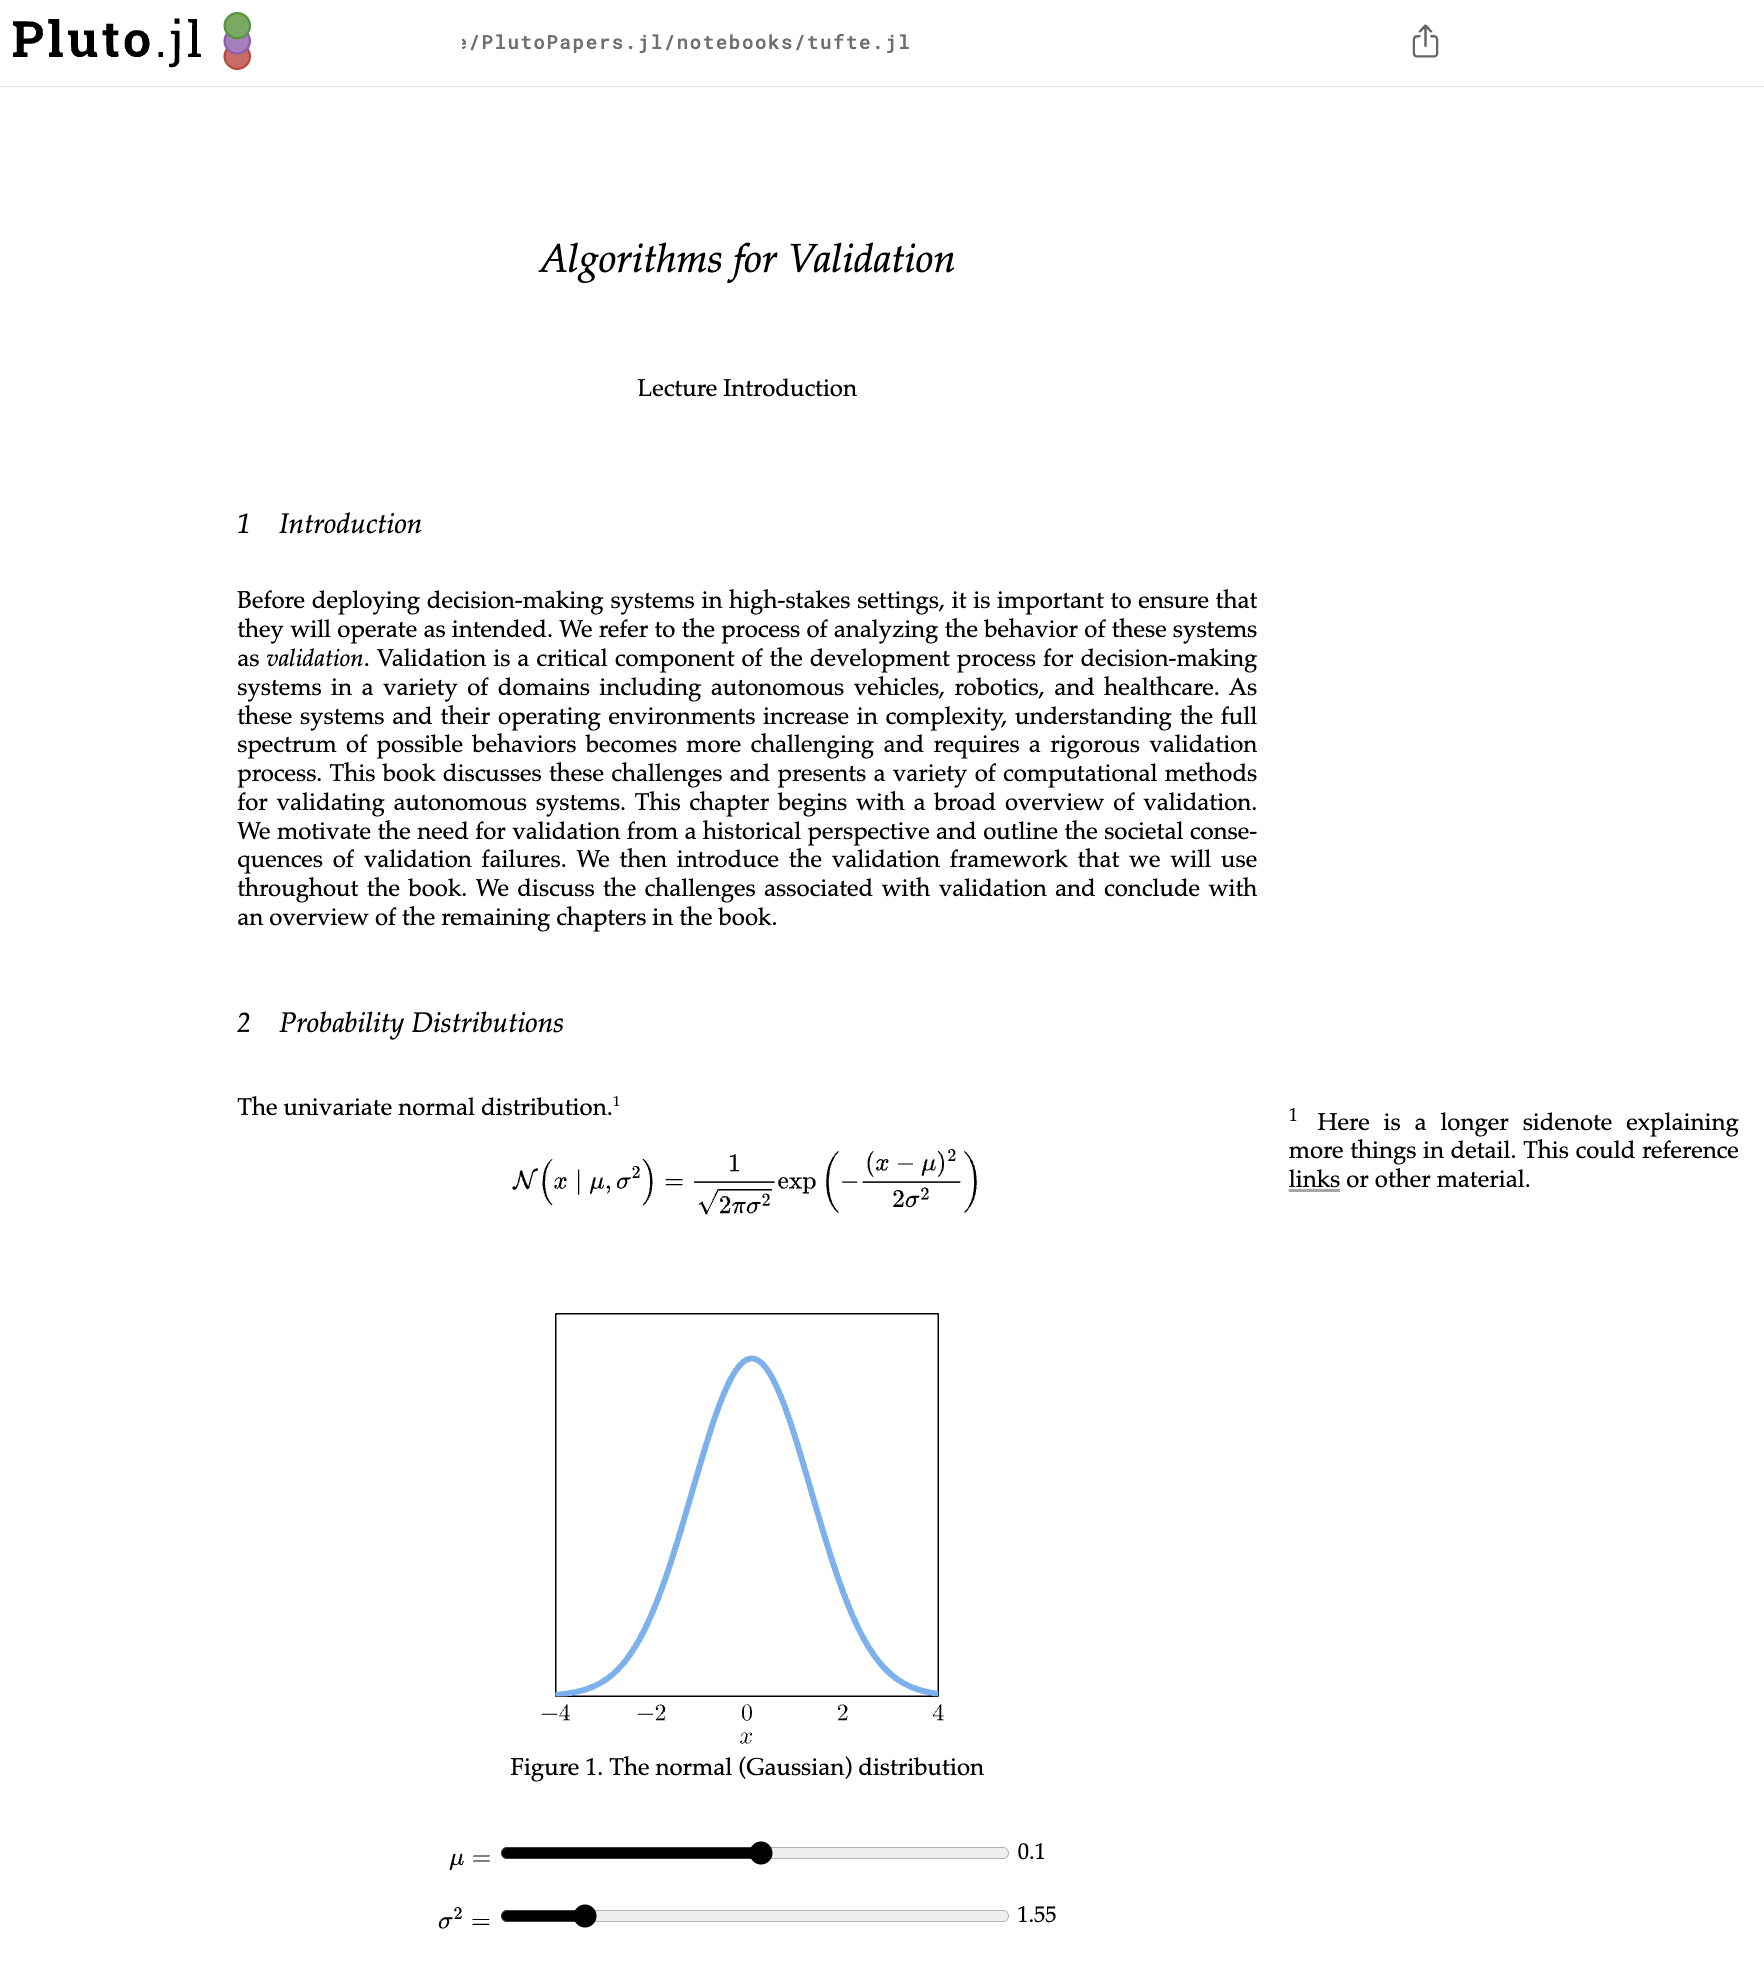
\includegraphics[width=\linewidth]{media/plutopapers-tufte-light.png}

    \captionof*{figure}{\shortstack{\footnotesize Interactive research papers\\\textcolor{gray}{\scriptsize Run code directly in the paper}}}
  \end{column}
  \pause
  \begin{column}{0.54\textwidth}
    
\includegraphics[width=0.85\linewidth]{media/PlutoPapers.jl.png}

    \textcolor{repo}{\small \url{https://github.com/mossr/PlutoPapers.jl}}
  \end{column}
  \hfill
\end{columns}
    
\end{frame}